\section{Ejercicio 1}
\subsection{Interpretación del enunciado}
\par{Se tiene una imprenta en la que cada día deben realizarse determinados
trabajos. Los trabajos son realizados por las máquinas de la imprenta. Esta
imprenta cuenta con dos máquinas idénticas. Los trabajos son distintos, pero
pueden ser realizados por cualquiera de la dos máquinas siempre que se repete
un orden dado. Las máquinas deben prepararse para realizar determinados
trabajos y estas preparaciones tienen un costo, el cuál depende tanto del
trabajo a realizar como del estado de la máquina. Teniendo los trabajos
ordenados y los costos de preparación de las máquinas para cada trabajo, se
debe tomar cada trabajo, elegir la máquina en la que se realizará ese trabajo,
prepararla, y realizar el trabajo. El objetivo del ejercicio es desarrollar un
algoritmo que determine la mejor distribución de los trabajos entre las
máquinas que reduzca el costo total de la operación, es decir la suma de los
costos de cada preparación.}

\subsection{Resolucion}
\par{Sea $p(j)$ el problema de obtener la distribución óptima de $j$ trabajos
entre $2$ máquinas, definimos el problema derivado $p'(j,i)$ con $0<i<j$, el
cual consiste en obtener la distribución óptima de $j$ trabajos entre $2$
máquinas con la restricción de que los últimos trabajos realizados en cada
máquina sean $t_j$ y $t_i$. Notar que es indiferente en qué máquina se ejecuta
cada uno de estos. Definimos entonces la $distribucionOptima(j,i$)
como la distribución de costo mínimo con $j$ trabajos y el
trabajo $t_i$ como último trabajo de una de las máquinas. Notar que cualquier
distribución de $j$ trabajos siempre va a tener a $t_j$ como último trabajo en
una de las máquinas. Luego, la solución para el problema $p(j)$ es la solución
de costo mínimo de $p(j,i)$ para todo $i$, es decir:}

$$p(j) = \min_{\forall i} p(j,i) $$

El problema $p'$ se resolvió con programación dinámica mediante $distribucionOptima(j,i)$, que se calcula de la siguiente manera:
$$distribucionOptima(j,i) = \left\{
\begin{array}{c l}
 costo(0,1) & j = 1\\
 distribucionOptima(j-1,0) + costo(j-1,j) & i = 0 \land j > 1\\
 distribucionOptima(j-1,i) + costo(j-1,j) & 1 \le i < j-1 \land j > 1\\
 \displaystyle \min_{\forall k} distribucionOptima(j-1,k) + costo(k,j) & i = j-1 \land j > 1\\
\end{array}
\right$$

\par{Notar que siempre $i < j$. La entrada para ambos problemas es la cantidad
de trabajos y los costos de preparación de las máquinas para cada trabajo
definidos como:}
\begin{equation*}
$costo($i$,$j$) = Costo de preparar una máquina para realizar el trabajo $t_j$ luego
de haber realizado el trabajo $t_i$ (o no haber realizado ningún trabajo si
$i=0$). $0 \leq i < j
\end{equation*}\\
\par{A continuación se muestra el pseudocódigo de la solución para $p(j)$,
resolviendo $p'(j,i)$.}\\
\begin{algorithm}[H]
	\caption{Algoritmo de Ejercicio 1}
	\KwData{\textbf{int} $cantTrabajos$, $costos$}
	$distribucionOptima(1,0) \longleftarrow costo(0,1)$\\
	\For{$j \in \{2..cantTrabajos\}$}{
		
		$distribucionOptima(j,0) \longleftarrow distribucionOptima(j-1,0) + costo(j-1,j)$\\
		$distribucionOptima(j,j-1) \longleftarrow distribucionOptima(j-1,0) + costo(0,j)$
		
		\For{$i \in \{1..j-2\}$}{
	
			$distribucionOptima(j,i) \longleftarrow distribucionOptima(j-1,i) + costo(j-1,j)$\\
			$distribucionOptima(j,j-1) \longleftarrow min(distribucionOptima(j,j-1), distribucionOptima(j-1,i) + costo(i,j))$\\
		}
	}
	\textbf{return} $ \displaystyle \min_{\substack{\forall i}} distribucionOptima(cantTrabajos,i) $\\
\end{algorithm}

\subsection{Demostración de Correctitud}

\textbf{Propiedad 1 -}  \emph{ Existe un $i$ tal que la solución del problema $p'(j,i)$
es solución de $p(j)$. }\\

\textbf{Demostración:} Es inmediato ver que alguna solución del problema $p(j)$ pertenece al
conjunto de las soluciones de $p(j,i)$ para algún $i$. Dado que $p(j)$ no tiene
la restricción del trabajo realizado como último en la otra máquina, la solución al
problema $p(j)$ es la solución de $p(j,i)$ con menor costo:
$$p(j) = \min_{\forall i} p(j,i)$$

\textbf{Propiedad 2 -} \emph{$ (\forall i < j) \quad distribucionOptima(j,i) $ devuelve una de las distribuciones con menor costo dados
j trabajos e i como último trabajo.}\\

\textbf{Demostración:}
Vamos a demostrar por inducción en j.


\textbf{Caso base. Si $j = 1:$}
Queremos ver que $ (\forall i < j) \quad distribucionOptima(1,i) $ devuelve una de las distribuciones con menor costo dados
$1$ trabajo e i como ultimo trabajo. Notar que siempre $i < j$ , por lo tanto $i$ debe ser $0$. 
Hay sólo una forma de configurar un trabajo en las dos máquinas, que este trabajo sea el único de una máquina
y la otra máquina este libre de trabajos, es decir que el costo de la distribución optima es igual a el costo de preparar
el trabajo $1$ luego del trabajo $0$ que es los mismo que \\
$distribucionOptima(1,0) = costo(0,1)$.
Luego, queda demostrado el caso base.\\


\textbf{Paso Inductivo:} Se dividirá la demostración en dos casos :\\

\textbf{Caso $i <  j-1$:} 

Definimos a $ distribucionOptima(j,i) $ = 
$distribucionOptima($j$-1,$i$) + costo($j$-1,$j$) & $\\
Supongamos que no es la distribución optima y lleguemos a un absurdo. Decir que es la distribución es óptima es lo mismo que afirmar que
que no hay ninguna distribución de $j$ trabajos con $i$ como último trabajo que cueste menos que $ distribucionOptima(j,i) $.
Sea $d_2$ la distribución que cuesta menos que $ distribucionOptima(j,i) $ y tiene j trabajos e i como último trabajo.
Luego por como se 
define la preparación de los trabajos,en $d_2$ el trabajo $j$ está al final de una máquina (y como $(i < j-1) \Rightarrow i \neq j $ )
y el trabajo $i$ está en la otra máquina. De esta manera, si quitamos el trabajo $j$, obtenemos una configuración de $j-1$ trabajos con $i$
como último trabajo, llamemosla $d_{2'}$.

\begin{align*}
\text{Por lo tanto}
\qquad costo (d_2) &= costo (d_{2'}) + costo(j-1,j) \\
\text{y como }
 \qquad costo(d_2) &<  distribucionOptima(j,i) \\ 
\text{entonces}
 \qquad costo (d_{2'}) &< distribucionOptima(j-1,i). Absurdo. 
\end{align*}

\textbf{Caso $i = j-1:$}

Definimos a $ distribucionOptima(j,i) $ =  
\displaystyle \min_{\substack{\forall i \in \{0..j-1\}}} \ $distribucionOptima($j$-1,$i$) + costo($i$,$j$)$
 & \\
 
Supongamos que no es la distribución optima y lleguemos a un absurdo.
Sea $d_2$ la distribución que cuesta menos que $ distribucionOptima(j,i) $ y tiene $j$ trabajos e $i$ como último trabajo.
Luego por como se 
define la preparación de los trabajos,en $d_2$ el trabajo $j$ está al final de una máquina (y como $(i = j-1) \Rightarrow i \neq j $ )
y el trabajo $i$ está en la otra máquina.
De esta manera, si quitamos el trabajo j, obtenemos una configuración de $j-1$ trabajos con $j-1$
y algún k (con $ 0 \le k < j-1$) como últimos trabajos en las dos máquinas, llamemosla $d_{2'}$.

\begin{align*}
\text{Por lo tanto}
\qquad costo (d_2) &= costo (d_{2'}) + costo(k,j)  \text{para algun k (con }  0 \le k < j-1) \\
\text{y como }
 \qquad costo(d_2) &<  distribucionOptima(j,i) \\ 
\text{entonces}
 \qquad costo (d_{2'}) &< distribucionOptima(j-1,k). 
\end{align*}

Absurdo pues por la definición
\displaystyle \min_{\substack{\forall k \in \{0..j-1\}}} \ $distribucionOptima($j$-1,$k$) + costo($k$,$j$)$. \\

\textbf{Corolario de Propiedad 2 -} \emph{$ distribucionOptima(cantTrabajos,i) $ devuelve una de las distribuciones con menor costo dados
cantTrabajos trabajos e i como ultimo trabajo.)}\\

Ahora veremos que el algoritmo retorna la distribución óptima según como la definimos.\\
\textbf{Caso $j = 1:$} En la línea $1$ del pseudocódigo se asigna la distribución óptima según como la definimos:
$$costo(1,0)$$
\textbf{Para $j > 1$:}
\textbf{Caso $i = 0$:} En la línea $3$ del pseudocódigo se asigna la distribución óptima según como la definimos:
$$distribucionOptima(j-1,0) + costo(j-1,j)$$
\textbf{Caso $1 \le i < j-1:$} En la línea $6$ del pseudocódigo se asigna la distribución óptima según como la definimos:
$$distribucionOptima(j-1,i) + costo(j-1,j)$$
\textbf{Caso $i = j-1:$} Sea $g(i) = distribucionOptima(j-1,i) + costo(i,j).$
En este caso se inicializa $distribucionOptima(j,j-1)$ en la linea $4$ con $g(0)$.
Luego en el ciclo interno se compara el valor actual de $distribucionOptima(j,j-1)$ con los valores
$g(i)$ para todo $ 1 \le i \le j-2 $. 


\subsection{Cota de Complejidad}
Para demostrar la complejidad del algoritmo, vemos que la incialización de la matriz de costos
tiene una complejidad de $O(n^2)$, con $n$ la cantidad de trabajos, ya que completa una matriz de $n^2$ elementos con dos ciclos anidados.

Luego, el algoritmo completa la matriz de $distribucionOptima$, con dos ciclos anidados. En cada uno de estos ciclos,
las variables de iteración se van incrementando de a uno y cada una debe iterar
en un numero menor o igual a la cantidad de trabajos.
\textbf{Cada asignación tiene una complejidad de $O(1)$, ya que al momento de la asignación (en la iteración $j$)
$distribucionOptima(j-1,i)$ ya está calculada y guardada en la matriz.}\\

\begin{algorithm}[H]
	\caption{Algoritmo de Ejercicio 1}
	\KwData{\textbf{int} $cantTrabajos$, $costos$}
	$distribucionOptima(1,0) \longleftarrow costo(0)(1)$	         \tcc*[r]{$O(1)$}
	\For{$j \in \{2..cantTrabajos\}$ \tcc*[r]{$O(n)$}}{	
		
		$distribucionOptima(j,0) \longleftarrow distribucionOptima(j-1)(0) + costo(j-1)(j)$\\ 	
		$distribucionOptima(j,j-1) \longleftarrow distribucionOptima(j-1)(0) + costo(0)(j)$		
		
		\For{$i \in \{1..j-2\}$ \tcc*[r]{$O(n)$} }{	
	
			$distribucionOptima(j,i) \longleftarrow distribucionOptima(j-1,i) + costo(j-1,j)$\\	${O(1)}$
			$distribucionOptima(j,j-1) \longleftarrow min(distribucionOptima(j,j-1), distribucionOptima(j-1)(i) + costo(i)(j))$\\
		}
	}
	\textbf{return} $ \displaystyle \min_{\substack{\forall i}} distribucionOptima(cantTrabajos,i) $	\tcc*[r]{$O(n)$}
\end{algorithm}

Luego la complejidad del algoritmos es $ O(n^2) + n * O(n) + O(n) = O(n^2).$

\subsection{Implementación}

\begin{lstlisting}
salida_ej1 resolver_ej1(entrada_ej1 entrada) {
  int cantTrabajos = entrada.n;
  vector<vector<int> > costo = entrada.matriz;

  //En la posicion i j está el costo de la configuración optima para
  //los primeros i trabajos con el trabajo j como ultimo de la otra máquina.
  vector < vector<par> > 
	distribucionOptima(cantTrabajos+1,vector<par> (cantTrabajos) );
  distribucionOptima[1][0] = make_pair(costo[0][1],0);
  
  for ( int j = 2; j <= cantTrabajos; ++j ) {
    distribucionOptima[j][0] = make_pair (distribucionOptima[j-1][0].first 
					+ costo[j-1][j],j-1);
    distribucionOptima[j][j-1] = make_pair (distribucionOptima[j-1][0].first
					+ costo[0][j],0);
    for ( int i = 1; i < j-1 ; ++i ) {
      distribucionOptima[j][i] = make_pair(distribucionOptima[j-1][i].first
						    + costo[j-1][j],j-1);
      int costoAlternativo = distribucionOptima[j-1][i].first + costo[i][j];
      if (costoAlternativo < distribucionOptima[j][j-1].first) {
	    distribucionOptima[j][j-1] = make_pair(costoAlternativo,i);
      }
    }
  }

  vector<int> tEnMaq1(0);
  int k = 0;
  int C = distribucionOptima[cantTrabajos][0].first;

  int elAnterior = cantTrabajos-1;
  int ultimoOtraMaquina = 0;
  for (int i=1; i<cantTrabajos; i++) {
      if (distribucionOptima[cantTrabajos][i].first < C) {
	C = distribucionOptima[cantTrabajos][i].first;
	elAnterior = distribucionOptima[cantTrabajos][i].second;
	ultimoOtraMaquina = i;
      }
  }
  
  //cout << "el anterior es " << elAnterior << endl;

  int trabajoEnMaquina = cantTrabajos;	
  tEnMaq1.push_back(trabajoEnMaquina);
  k++;

  while (elAnterior != 0){
    tEnMaq1.push_back(elAnterior);
    k++;
    trabajoEnMaquina = elAnterior;
    while (ultimoOtraMaquina > elAnterior) {
      ultimoOtraMaquina = 
	      distribucionOptima[ultimoOtraMaquina][elAnterior].second;
      }
    elAnterior = 
	distribucionOptima[trabajoEnMaquina][ultimoOtraMaquina].second;
}

  vector<int> e = vector<int>(k);
  for (int i=0; i<k; i++) {
	  e[i] = tEnMaq1[k-i-1];
  }

  //cout << "vector de trabajos" << endl;
  //mostrarVec(e);
  
  //cout << "matriz de cofiguracion Optima" << endl;
  //mostrarMatriz(distribucionOptima,cantTrabajos+1,cantTrabajos);
  //cout << endl;

  salida_ej1 salida(C, k, e);
  return salida;
}
\end{lstlisting}
\newpage
\subsection{Testing de Correctitud}

Los tests expuestos a continuación fueron diseñados con el fin de verificar
diferentes casos particulares que pudimos identificar. Para cada test vamos
a exponer la entrada, la salida y, en caso de que sea necesario, una
justificaci\'on de la correctitud de la soluci\'on.\\

\noindent\textbf{Test$\#$1}\\
\textbf{Caracterización:} Un solo trabajo.\\
\textbf{Input:}\\ \texttt{1\\5}\\
\textbf{Output:} \texttt{5 1 1}\\
\textbf{Status:} OK. Asigna el único trabajo a la máquina 1 y el costo total
es el costo de ubicar el trabajo 1 en la máquina 1.\\

\noindent\textbf{Test$\#$2}\\
\textbf{Caracterización:} Dos trabajos que conviene ubicar uno trás otro.\\
\textbf{Input:}\\ \texttt{2\\3\\8 3}\\
\textbf{Output:} \texttt{6 2 1 2}\\
\textbf{Status:} OK. Ubica ambos trabajos en la misma máquina y el costo
total es el costo de ubicar el trabajo 1 en una máquina vacía más el costo
de ubicar el trabajo 2 tras el trabajo 1.\\

\noindent\textbf{Test$\#$3}\\
\textbf{Caracterización:} Dos trabajos que conviene ubicar como primeros en
una máquina.\\
\textbf{Input:}\\ \texttt{2\\3\\3 8}\\
\textbf{Output:} \texttt{6 1 2}\\
\textbf{Status:} OK. Ubica un trabajo en cada máquina y el costo total es la
suma de los costos de ubicar cada trabajo como primer trabajo de una máquina.\\

\noindent\textbf{Test$\#$4}\\
\textbf{Caracterización:} Todos los costos son iguales.\\
\textbf{Input:}\\ \texttt{5\\1\\1 1\\1 1 1\\1 1 1 1\\1 1 1 1 1}\\
\textbf{Output:} \texttt{5 5 1 2 3 4 5}\\
\textbf{Status:} OK. Cualquier distribución de trabajos en máquinas tiene
costo igual a 5.\\

\noindent\textbf{Test$\#$5}\\
\textbf{Caracterización:} Todos los costos son distintos (incrementando).\\
\textbf{Input:}\\ \texttt{3\\1\\2 3\\4 5 6}\\
\textbf{Output:} \texttt{8 1 3}\\
\textbf{Status:} OK.\\

\noindent\textbf{Test$\#$6}\\
\textbf{Caracterización:} Todos los costos son distintos (decrementando).\\
\textbf{Input:}\\ \texttt{3\\6\\5 4\\3 2 1}\\
\textbf{Output:} \texttt{11 3 1 2 3}\\
\textbf{Status:} OK.\\

\noindent\textbf{Test$\#$7}\\
\textbf{Caracterización:} Varios trabajos que conviene ubicar uno tras otro.\\
\textbf{Input:}\\ \texttt{5\\1\\8 1\\8 8 1\\8 8 8 1\\8 8 8 8 1}\\
\textbf{Output:} \texttt{5 5 1 2 3 4 5}\\
\textbf{Status:} OK. Ubica todos los trabajos en la misma máquina.\\

\noindent\textbf{Test$\#$8}\\
\textbf{Caracterización:} Varios trabajos que conviene ubicar intercalados.\\
\textbf{Input:}\\ \texttt{5\\1\\1 8\\8 1 8\\8 8 1 8\\8 8 8 1 8}\\
\textbf{Output:} \texttt{5 3 1 3 5}\\
\textbf{Status:} OK. Ubica los trabajos impares en la misma máquina (por lo
tanto, ubica los pares en la otra).\\

\noindent\textbf{Test$\#$9}\\
\textbf{Caracterización:} La subsolución de la solución óptima no es solución
óptima para su subproblema asociado.\\
\textbf{Input:}\\ \texttt{3\\5\\3 5\\1 8 8}\\
\textbf{Output:} \texttt{11 1 3}\\
\textbf{Status:} OK. La solución óptima consiste en ubicar los trabajos 1 y 2 en
una máquina y el trabajo 3 en otra. Sin embargo, la subsolución de dos trabajos
que ubica a los trabajos 1 y 2 en la misma máquina no es solución óptima del
subproblema asociado (distribuír los trabajos 1 y 2 entre las 2 máquinas de
forma óptima.)\\

\newpage
\subsection{Testing de Performance}

\par{Realizamos un gráfico comparando la sucesión de tiempos obtenida con una función cuadrática, pues demostramos que la complejidad del algoritmo es cuadrática.
La función $f = n^2$, donde $C = \frac{1}{20500000}$. Se midió el tiempo con n desde 1 hasta 1000 con saltos de a 10 (con 100 mediciones por cada n).}


\begin{figure}[H]
\centering
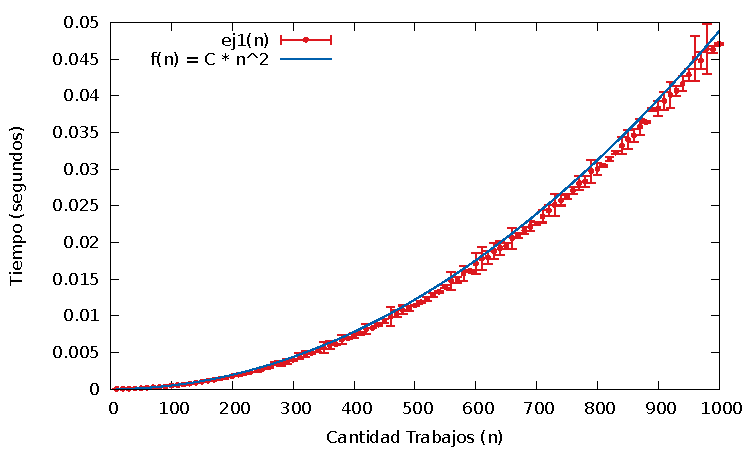
\includegraphics{imgs/ej1_1000_10_100.pdf}
\caption{Test Performance: Tiempo(s) vs Cantidad de Trabajos.}
\end{figure}

\par{Hay que notar que las franjas para cada tamaño de entrada muestran el desvío estandar de todos los valores conseguidos para ese tamaño, esto nos pareci\'o mucho m\'as significativo que simplemente mostrar el máximo y el m\'inimo, ya que estos valores pueden variar mucho por otros procesos que pueda estar ejecutando la computadora a la vez.}
